\documentclass[a4paper]{article}
\usepackage[a4paper,top=1cm,bottom=2cm,left=2cm,right=2cm,marginparwidth=1.75cm]{geometry}
\usepackage{amsmath}
\usepackage{graphicx}
\usepackage{amssymb}
\usepackage[colorlinks=true, allcolors=blue]{hyperref}

\title{\textbf{EN2550 - Fundamentals of Image Processing and Machine Vision}\\
Assignment 02}
\author{Tharindu O.K.D.\\19062R}
\begin{document}
\maketitle
GitHub Repository : \url{https://github.com/dakshinatharindu/Image-Processing/blob/main/Assignment-02/190622R_a02.ipynb}

\section*{Question 01}
\begin{figure}[!htb]
    \centering
    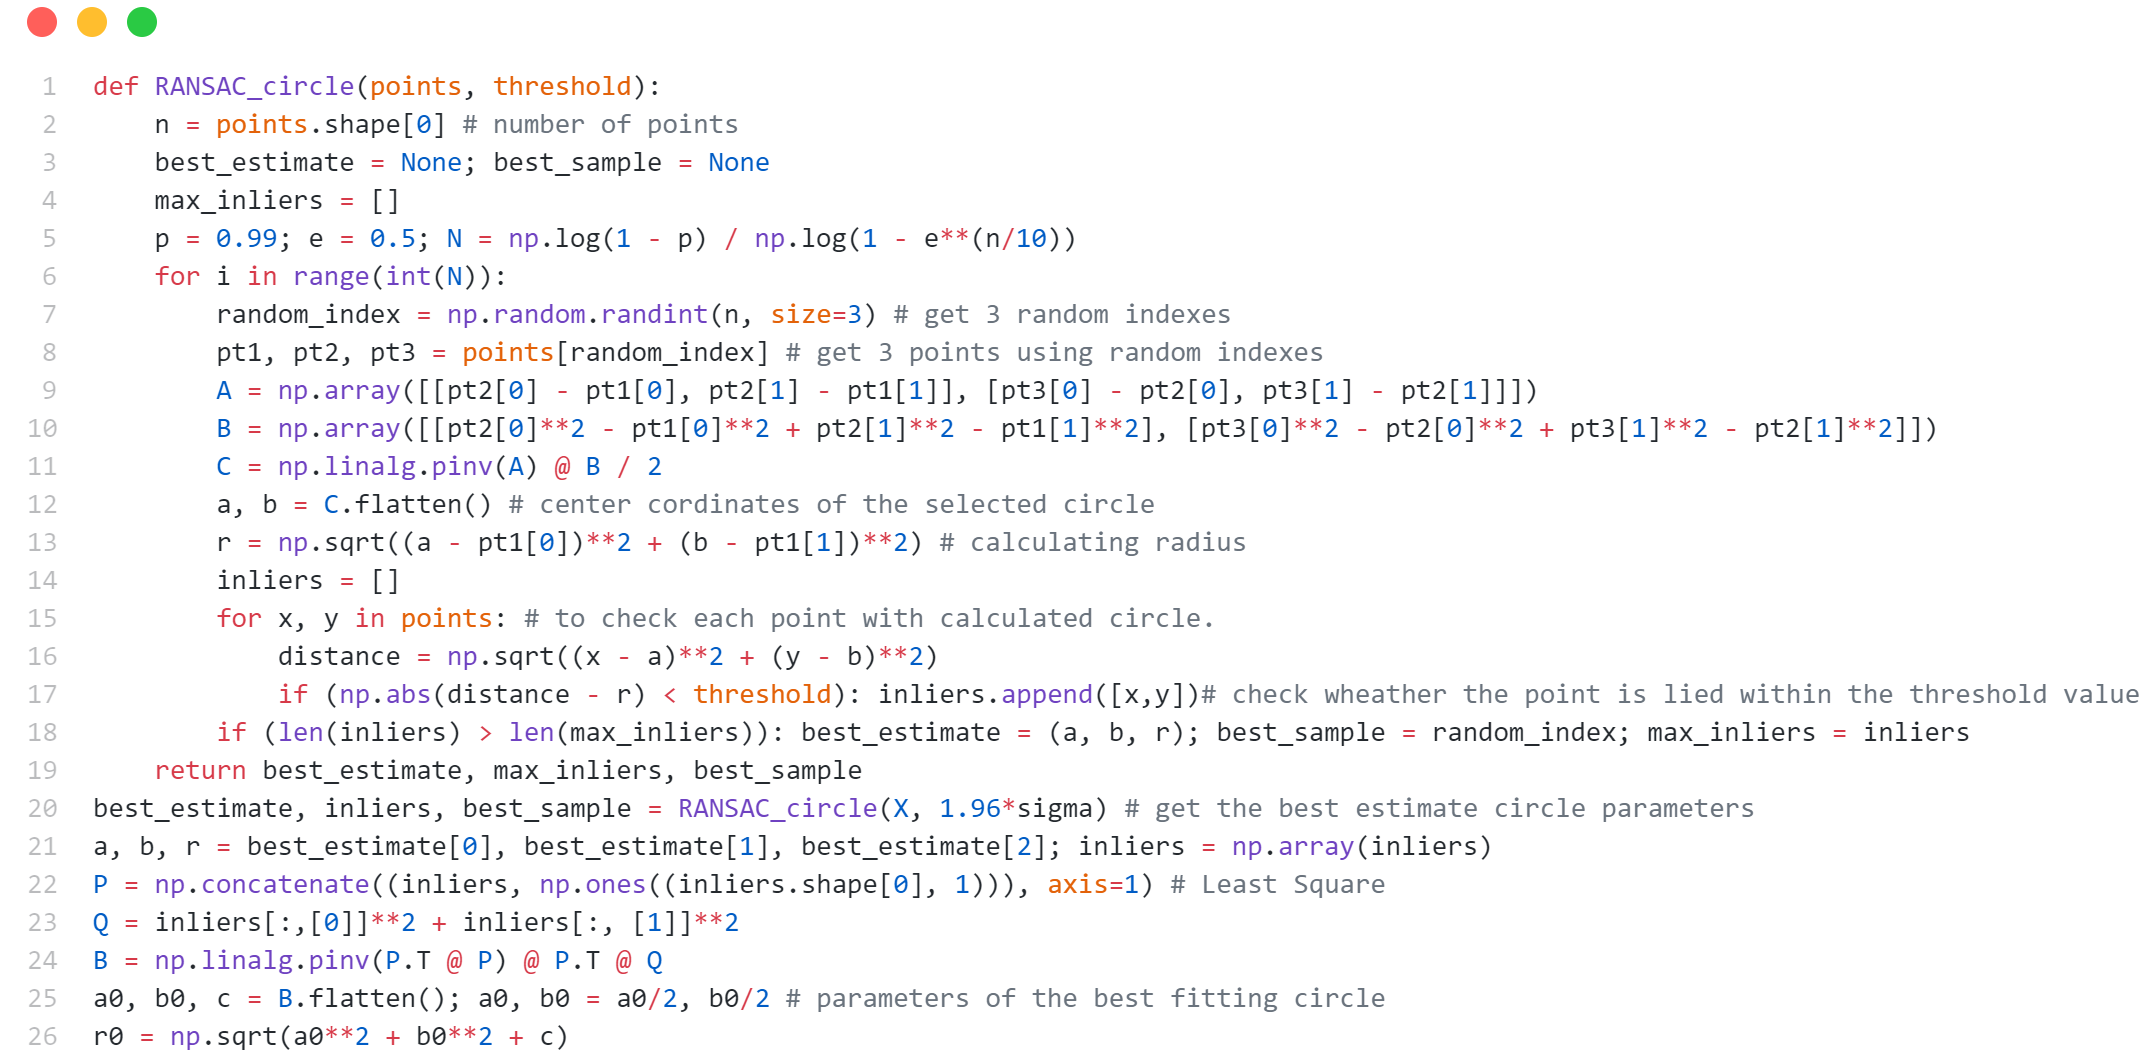
\includegraphics[width=\textwidth]{images/ransac_circle.png}
    \caption{$RANSAC\_circle$ function}
    \label{ransac_circle}
\end{figure}
Our objective of this function is to robustly fit a circle to our point set. This can be done using RANSAC
algorithm. Figure 1 shows the code snipped of the RANSAC function.
 
\subsubsection*{RANSAC Algorithm Explanation}
\begin{enumerate}
  \item First, we calculate the number of iterations $N$ required to get a better estimation. We choose $N$ 
  so that, with probability $p$, at least one random sample is free from outliers.
  It is given by, $N=\frac{\log{(1-p)}}{\log{(1-(1-e)^n)}}$. Here $e$ is outlier
  ratio and $n$ is a number of points. Here I took $e=0.5$ and $p=0.99$ so 
  that 50\% of points will fall into inliers with a 99\% probability.
  \item We randomly select 3 points from the given data set. Then we calculate the fitting
   circle using these 3 points as follows.
   $$(x-a)^2+(y-b)^2=r^2$$substituting 3 point coordinates and putting it into matrix form, we get
   \begin{align*}
     \begin{pmatrix}
       x_2-x_1 & y_2-y_1\\
       x_3-x_2 & y_3-y_2
     \end{pmatrix}
     \begin{pmatrix}
       2a\\
       2b
     \end{pmatrix}&=
     \begin{pmatrix}
      x_2^2-x_1^2 & y_2^2-y_1^2\\
      x_3^2-x_2^2 & y_3^2-y_2^2
    \end{pmatrix}\\
    AC&=B\\
    C&=A^{-1}B
   \end{align*}
   Then we can find center coordinates and radius using the $C$ matrix.
   \item Then determine the inlier set 
   $$inliers=\{(x_i,y_i)\in points \text{ such that }|\sqrt{(x_i-a)^2+(y_i-b)^2}-r|<threshold\}$$
   \item If $|inliers|>|max\_inliers|$, we select it as the best estimate. Go to step 2
   until iterate N times.
  \end{enumerate}

  \subsubsection*{Finding Best Fitting Circle}

\begin{figure}[!htb]
  \centering
  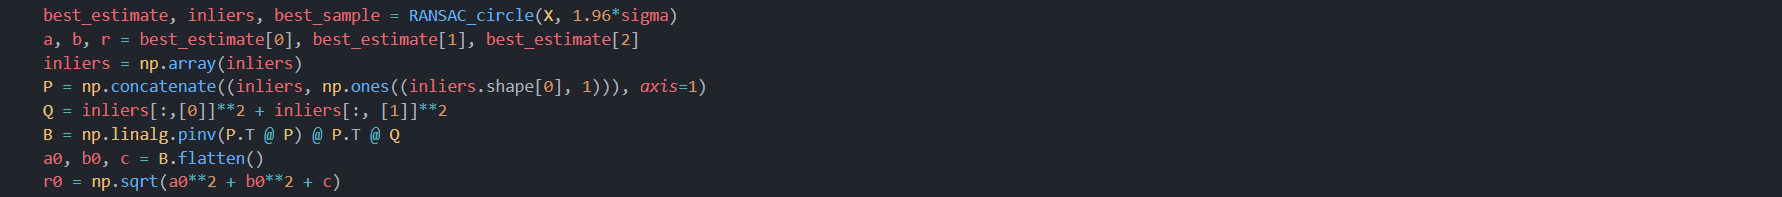
\includegraphics[width=\textwidth]{images/best_fit.png}
  \caption{Finding Best Fitting Circle}
  \label{bestfit}
\end{figure}
First, we get the parameters of the best fitting circle using the above 
$RANSAC\_circle$ function. Since the sample noise is distributed as zero-mean
 Gaussian, we pass the threshold value as $1.96\sigma$ so that will give
  a $\approx95\%$ probability of capturing all inliers. After
   finding the best inliers, we find the best fitting circle for
    those inliers using the Least Square approach as follows.
    \begin{align*}
      \begin{pmatrix}
        x_1 & y_1 & 1\\
        x_2 & y_2 & 1\\
        \vdots & \vdots & \vdots\\
        x_n & y_n & 1\\
      \end{pmatrix}
      \begin{pmatrix}
        2a_0 \\ 2b_0 \\ c
      \end{pmatrix}&=
      \begin{pmatrix}
        x_1^2 & y_1^2\\
        x_2^2 & y_2^2\\
        \vdots & \vdots \\
        x_n^2 & y_n^2\\
      \end{pmatrix}\\
      PB&=Q\\
      B&=(P^T P)^{-1}P^T Q
    \end{align*}
    Using the B matrix, we can find
     $a_0, b_0$, and $r_0$ which are the parameters of the best-fitting
      circle.
\begin{figure}[!htb]
  \centering
  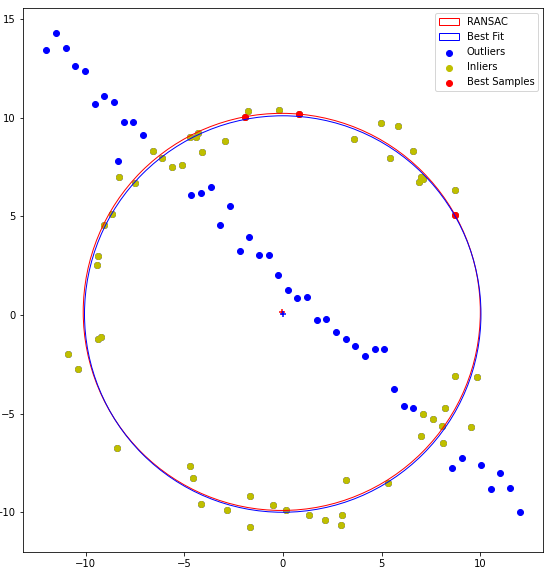
\includegraphics[width=0.5\textwidth]{images/ransac.png}
  \caption{Output}
  \label{ransac}
\end{figure}
\section*{Question 02}
\begin{figure}[!htb]
  \centering
  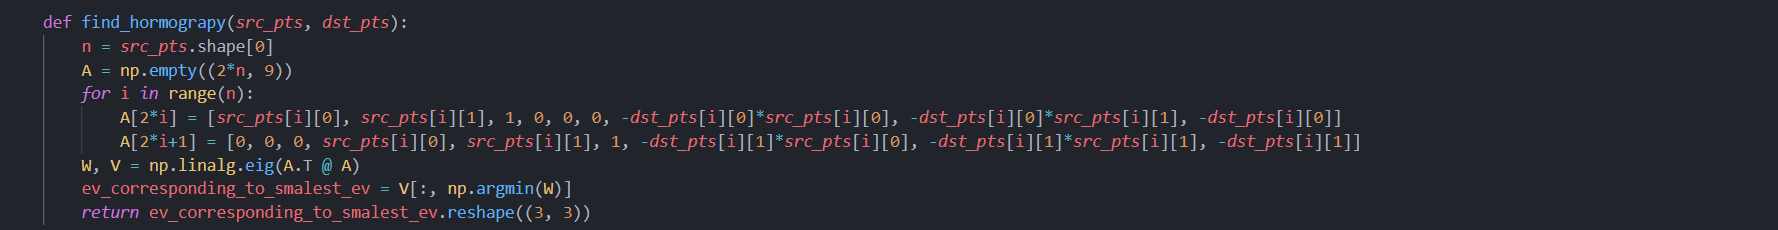
\includegraphics[width=\textwidth]{images/find_hormo.png}
  \caption{find\_hormography Function}
  \label{find_hormography}
\end{figure}

\begin{figure}[!htb]
  \centering
  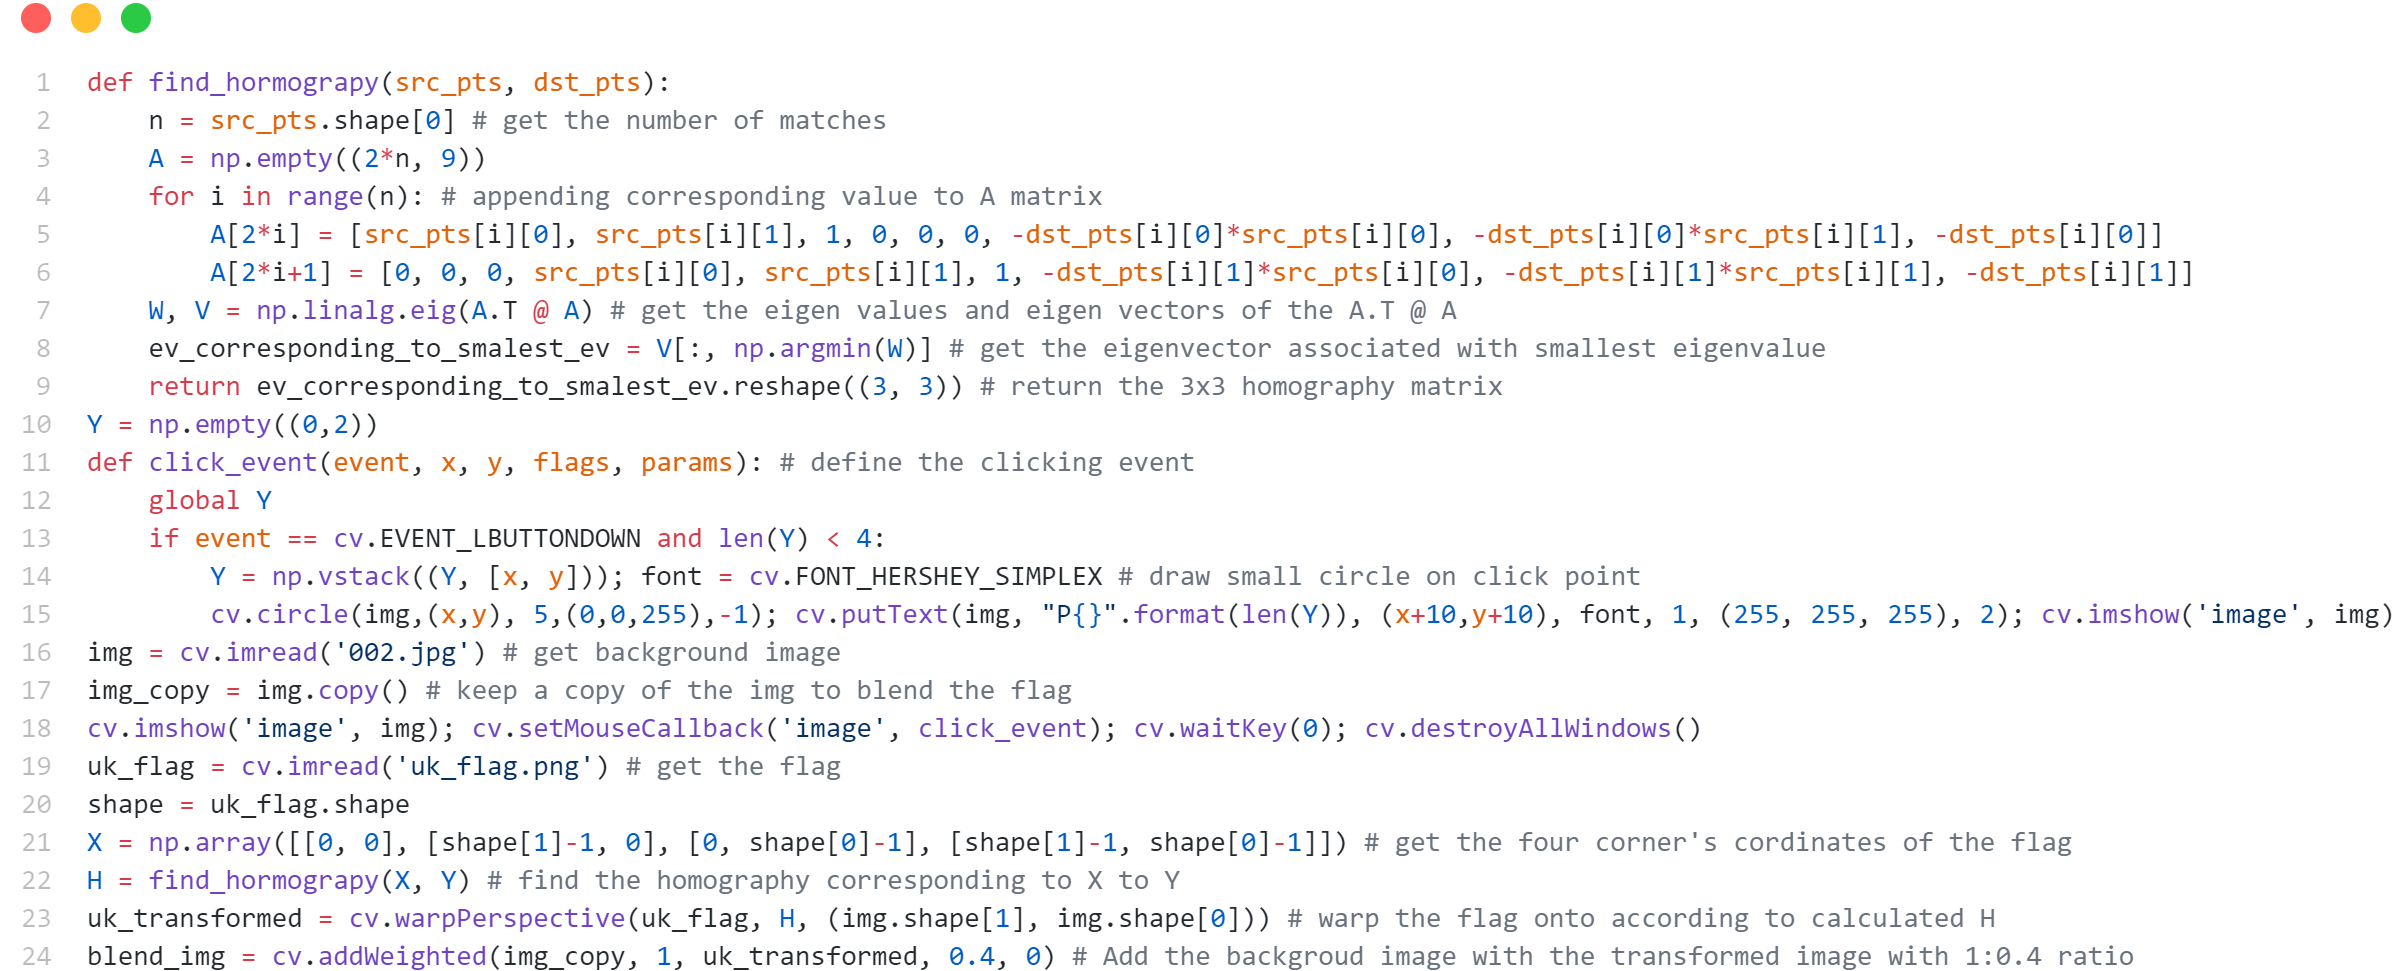
\includegraphics[width=\textwidth]{images/q2code.png}
  \caption{Code}
  \label{q2code}
\end{figure}
\subsubsection*{Algorithm Explanation}
\begin{enumerate}
  \item First, we find the coordinates of the selected points ($Y$) using
   mousing clicking and find the coordinates of the four corners($X$) of
    the flag. Then we feed these source points ($X$) and destination points
     ($Y$) to the $find\_homography$ function as shown in Figure \ref{find_hormography}.
  \item Although, we only need four correspondences to find the
   homography matrix, in this function, if we give more than four
    points it will calculate the homography matrix using the least
     square approach  ($\because$ this will be required for question 03). This
      will not be a problem because if we give the exact four
       correspondences, it will return the exact homography matrix.
        In the $find\_homography$ function,
   we put each coordinate into matrix form as shown below.
   \begin{align*}
     \begin{pmatrix}
       \vdots & \vdots & \vdots & \vdots & \vdots & \vdots & \vdots & \vdots & \vdots\\
       x_s^{(i)} & y_s^{(i)} & 1 & 0 & 0 & 0 &-x_d^{(i)}x_s^{(i)} &-x_d^{(i)}y_s^{(i)} & x_d^{(i)}\\
       0 & 0 & 0 & x_s^{(i)} & y_s^{(i)} & 1 & -y_d^{(i)}x_s^{(i)} &-y_d^{(i)}y_s^{(i)} & y_d^{(i)}\\
       \vdots & \vdots & \vdots & \vdots & \vdots & \vdots & \vdots & \vdots & \vdots
     \end{pmatrix}
     \begin{pmatrix}
       h_{11} \\ h_{12} \\h_{13} \\ h_{21} \\ h_{22} \\ h_{23} \\ h_{31} \\ h_{32} \\ h_{33}
     \end{pmatrix}&=
     \begin{pmatrix}
       \vdots \\ 0 \\ \vdots
     \end{pmatrix}\\
   \end{align*}
   $$Ah=0$$
   Since $H$ is defined up to a scale value, we can solve
    this as a Constrained Least
     Square problem. i.e. $h$ is 
     the eigenvector associated with the smallest eigenvalue
      of the matrix $A^TA$. Then we can find the $H$ matrix using $h$ vector.
    \item After finding the homography matrix, we can use the
     OpenCV warpPerspective
      method to warp the flag into selected points.
       To blend the two images, I have used the OpenCV
        addWeighted method which will add the two images with
         a given ratio.
    \end{enumerate}
Figure \ref{q2} shows selected points in the order and the resulting
     image for the UK flag and Sri Lanka flag.


\begin{figure}[!htb]
  \centering
  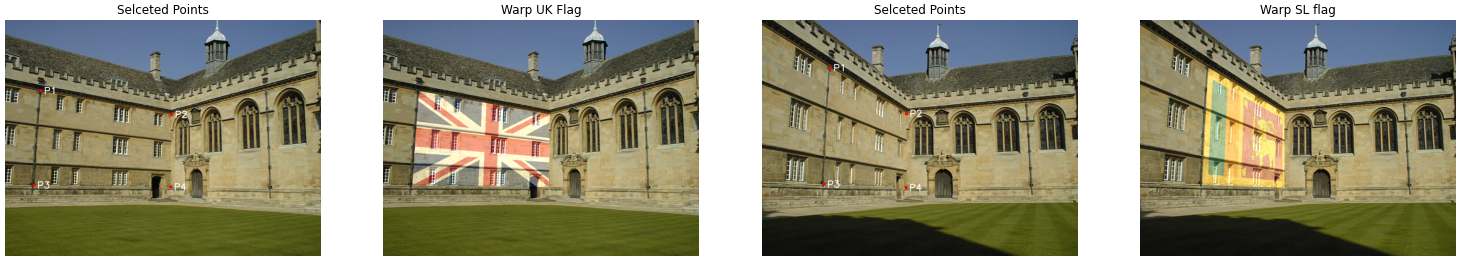
\includegraphics[width=\textwidth]{images/q22.png}
  \caption{Output}
  \label{q2}
\end{figure}
\end{document}
